\section{Auswertung}
\label{sec:Auswertung}
\subsection{Charakteristik des Geiger-Müller-Zählrohrs}
\label{subsec:auscharak}
Die Messwerte die wie in Abschnitt \ref{subsec:charak} beschrieben, aufgenommen wurden sind in Tabelle \ref{tab:imps} aufgelistet worden.
In der Abbildung \ref{fig:imps} wurden diese grafisch aufgetragen.
Die Grafik wurde mit dem python Plugin matplotlib \cite{matplotlib} erstellt.
Dabei ergibt sich der Fehler der Werte aus $\Delta N = \sqrt{N}$.
In der Grafik  ist ebenfalls eine Ausgleichsgerade zu sehen.
Diese wurde mit dem python Plugin scipy \cite{scipy} erstellt.
Die Werte mit denen die Ausgleichsgerade berechnet wurden, sind dabei die Werte die das Plateau bilden.
Zur Bestimmung der Qualität des Zählrohrs wurde nun die Steigung des Plateaus mithilfe der zuvor genannten Ausgleichsgeraden angenähert.
Dazu wurde diese nach dem Muster 
\begin{equation*}
  N(U)=aU+b
\end{equation*} 
erstellt.
Die Wert der Steigung $a$ und der Wert $b$ sind dabei
\begin{align*}
  a &= \SI{1.16(22)}{\frac{\text{Imp}}{\V}} \\
  b &= \SI{9.58(11)e03}{\text{Imp}}.\\
\end{align*}
Die relative Steigung kann durch
\begin{align*}
    \Delta N_\text{rel} &= \left( \frac{N(U=\SI{640}{\volt})}{N(U=\SI{370}{\volt})} - 1 \right) \cdot \frac{\SI{100}{\volt}}{(640-370)\:\si{\volt}} \cdot 100 \\
             &= \SI{1.7(5)}{\percent\per100\volt}
\end{align*}
bestimmt werden.
\begin{figure}
  \centering
  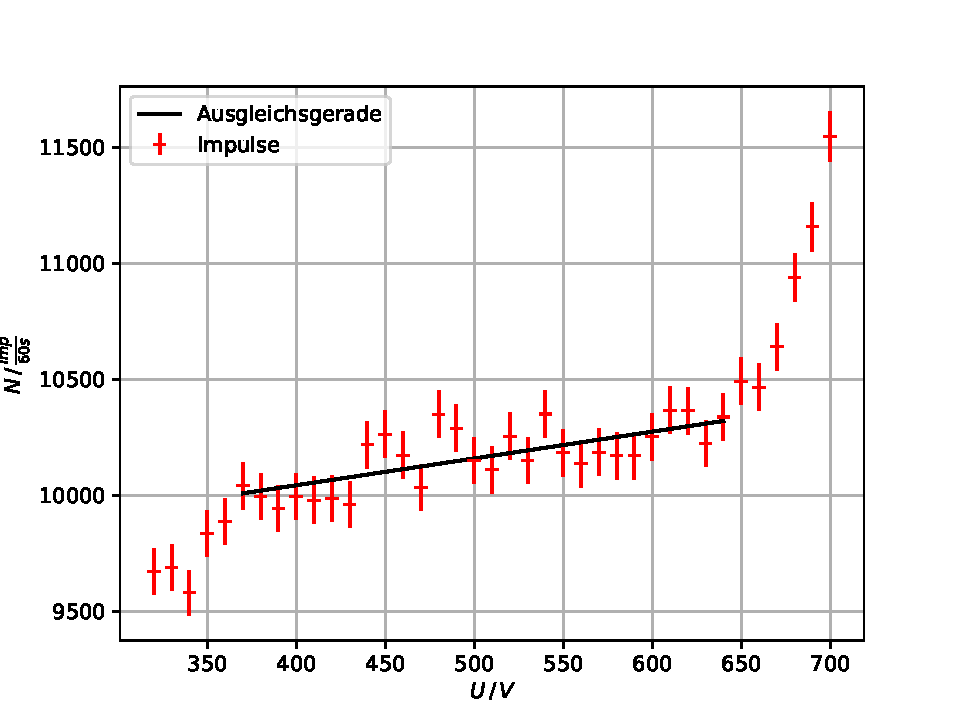
\includegraphics[width=0.6\textwidth]{content/data/kennlinie.pdf}
  \caption{Die aufgenommenen Messwerte mit zugehörigen Fehlern, sowie die Ausgleichsgerade im Plateau.}
  \label{fig:imps}
\end{figure}

\begin{table}
  \centering
  \caption{Die gemessenen Impulse pro $60\si{\second}$ in Abhängigkeit von der Spannung am Zählrohrs.}
  \begin{tabular}[t]{cc}
    \toprule
    $U \, /\, \si{\V}$ & $N \,/\, \frac{\text{Imp}}{\si{60\second}}$\\
    \midrule
    320 & 9672    \\
    330 & 9689    \\
    340 & 9580    \\
    350 & 9837    \\
    360 & 9886    \\
    370 & 10041   \\
    380 & 9996    \\
    390 & 9943    \\
    400 & 9995    \\
    410 & 9980    \\
    420 & 9986    \\
    430 & 9960    \\
    440 & 10219   \\
    450 & 10264   \\
    460 & 10174   \\
    470 & 10035   \\
    480 & 10350   \\
    490 & 10290   \\
    500 & 10151   \\
    510 & 10110   \\
    \bottomrule
  \end{tabular}
  \begin{tabular}[t]{cc}
    \toprule
    $U \, /\, \si{\V}$ & $N \,/\, \frac{\text{Imp}}{\si{60\second}}$\\
    \midrule
    520 & 10255   \\
    530 & 10151   \\
    540 & 10351   \\
    550 & 10184   \\
    560 & 10137   \\
    570 & 10186   \\
    580 & 10171   \\
    590 & 10171   \\
    600 & 10253   \\
    610 & 10368   \\
    620 & 10365   \\
    630 & 10224   \\
    640 & 10338   \\
    650 & 10493   \\
    660 & 10467   \\
    670 & 10640   \\
    680 & 10939   \\
    690 & 11159   \\
    700 & 11547   \\
    \bottomrule
  \end{tabular}
\label{tab:imps}
\end{table}
\FloatBarrier
\subsection{Totzeitberechnung}
Zur Berechung der Totzeit wurden die drei Werte
\begin{align*}
  N_1 &= \SI{96041}{\frac{\text{Imp}}{120\second}} \\
  N_{1+2} &= \SI{158479}{\frac{\text{Imp}}{120\second}} \\
  N_2 &= \SI{76581}{\frac{\text{Imp}}{120\second}} \\
  \label{eq:tot}
\end{align*}
aufgenommen.
Der Prozess der Messung ist in Abschnitt \ref{subsec:tot} beschrieben worden.
Mit diesen Werten kann mit Hilfe von Gleichung \eqref{eq:totzeit} die Totzeit $T$ des Geiger-Müller-Zählrohrs bestimmt werden.
Bei dem genutzten Zählrohr lässt sich die Totzeit auf 
\begin{equation*}
    T = \SI{115+-4}{\micro\second} \, .
\end{equation*}
bestimmten.
Zudem wurde versucht die Totzeit durch ablesen an einem Osziloskop zu bestimmen.
Die Peaks sind auf dem Bild nicht gut zu erkennen, dennoch lässt sich die Totzeit durch diese Methode auf
\begin{equation*}
  T \approx 100 \si{\micro\second}
\end{equation*}
bestimmen.
\FloatBarrier
\subsection{Freigesetzte Ladung pro eingefallenem Teilchen}
Zur Berechnung der freigesetzten Ladung pro eingefallenem Teilchen wurde während der Messung der Impulse, in Abschnitt \ref{subsec:charak} beschrieben, auch die Stromstärke $I$ am Geiger-Müller-Zählrohr gemessen.
Die gemessenen Stromstärken sind in der Tabelle \ref{tab:strom} zusammen mit den jeweilgen Impulswerten zu sehen.
Aus diesen lassen sich mit der Gleichung \eqref{eq:z} die Zahl $Z$ berechnen, welche angibt wie viele Ladungen durch ein einfallendes Teilchen freigesetzt wurden.
Aus den berechneten Werten wurde im folgenden ein Plot erstellt, dieser ist in Abbildung \ref{fig:z} zu sehen.
Die Regressionsgerade wurde nach dem Schema $f(x)=Ua+b$ erstellt.
Der Wert der Steigung $a$ entspricht dabei der gesuchten Zahl $Z$.
Die Werte für $a$ und $b$ entsprechen
\begin{align*}
  a &= \SI{1.37(6)e+14}{} \\
  b &= \SI{-3.78(31)e+16}{}
\end{align*}
\begin{table}
  \centering
  \caption{Die gemessenen Stromstärken und Spannungen zu den passenden Impulswerten, zudem die berechneten Werte für $Z$ mit Unsicherheiten.}
  \begin{tabular}[t]{ccccc}
    \toprule
    $U\,/\, \si{V} $ &$I \, /\, \si{\A}$ & $N \,/\, \frac{\text{Imp}}{\si{60\second}}$& $Z\cdot\SI{e16}{}$ & $\Delta Z\cdot\SI{e16}{}$\\
    \midrule
    350 & 0.3 & 9837  & 1.14 & 0.19 \\
    400 & 0.4 & 9995  & 1.50 & 0.19 \\
    450 & 0.7 & 10264 & 2.55 & 0.18  \\
    500 & 0.8 & 10151 & 2.95 & 0.19  \\
    550 & 1.0 & 10184 & 3.68 & 0.19  \\
    600 & 1.3 & 10253 & 4.75 & 0.19  \\
    650 & 1.4 & 10493 & 5.00 & 0.18  \\
    700 & 1.8 & 11547 & 5.84 & 0.17  \\
    \bottomrule
    \end{tabular}
  \label{tab:strom}
\end{table}

\begin{figure}
  \centering
  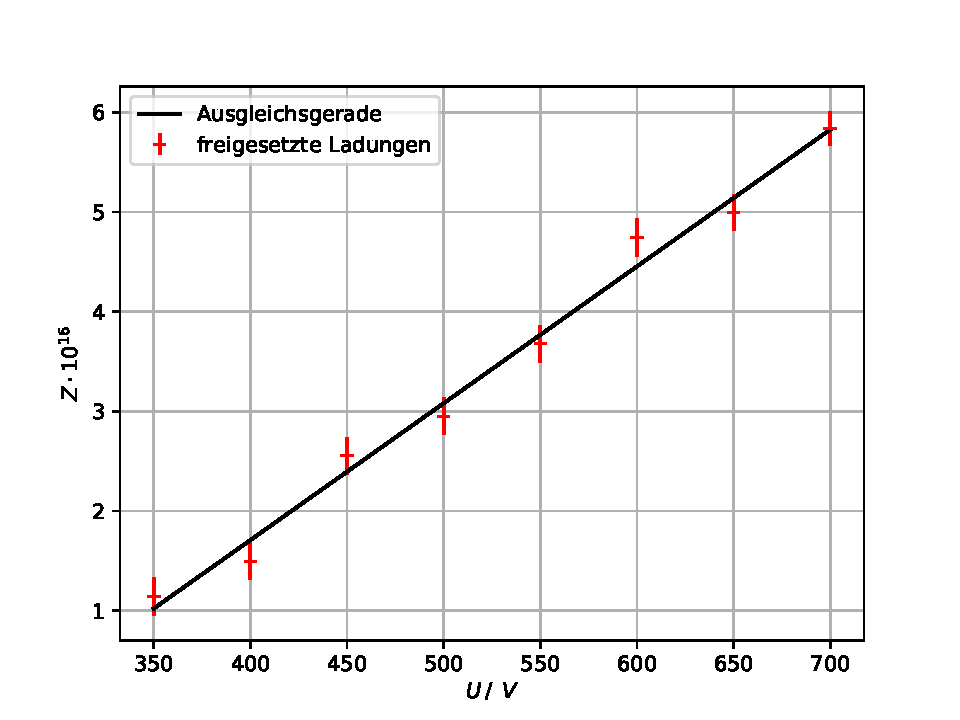
\includegraphics[width=0.6\textwidth]{content/data/zaehlstrom.pdf}
  \caption{Die Zahl der freigesetzten Ladungen pro Teilchen $Z$ aufgetragen gegen die Spannung $U$.}
  \label{fig:z}
\end{figure}